\documentclass{article}
\usepackage[utf8]{inputenc}
\usepackage{graphicx}
\graphicspath{ {images/} }
\usepackage[letterpaper, portrait, margin=1.5in]{geometry}

\renewcommand{\baselinestretch}{2}

\title{Color}
\author{Kesley Copley }
\date{December 2015}

\begin{document}

\maketitle

\begin{abstract}
This is just filler text so I can see whether the abstract looks okay. I'm going to type a little more. Wow, I really hope I don't forget to come back and add an actual abstract. That would be unfortunate. Okay, why is this thing indented? I don't like it. Make it stop. 
\end{abstract}

\section{Introduction}
\paragraph
\indent This is more filler text so I don't have an empty thing, but this will be my introduction. It will be written after I've completed the paper and before I write the conclusion and abstract. Yes, blah, blah, blah. This is a lot of filler text to try and make images work becasue for some reason, they aren't. 

\section{What is color?}
\paragraph
\indent Color is a fundamental part of the human experience. Everyday the human brain receives information about the world and has to make sense of the input. That sensory data comes from the skin, the eyes, the ears, the nose, and the tongue. In the case of seeing color, light is reflected off an object. It’s wavelengths are then picked up by the color receptors in the eyes. Cone cells in the eyes detect red, blue, and green light. The visual information travels to the brain through the optic nerve. It is then interpreted by the brain and stored for later reference. The average human being does not know how much light is being reflected when they look at a firetruck or a school bus. They see what they have been taught to understand is red and yellow. And without the parts of the eyes that distinguish saturation and color, literally everything would be different. Without color, humans would not know that a banana has passed its ripe period or when a pepper is ready to pick. Humans would not be able to tell the difference between a venomous snake or one that’s harmless. Not only is color important to humans, but to other animals as well. Hummingbirds, for example, are attracted to the color red because that is the color they associate with flowers, so many hummingbird feeders are red to attract more of the birds. Also, the male hummingbirds have brightly colored necks to get the attention of a possible mate, while females have more muted colors to act as a camouflage from predators.
\paragraph
\indent Color is a tool, a way of expressing feeling and generating emotion. Color is a sensational experience that will change the way people see something. Color is specifically artificial and pigmentation; it is created and prone to change. I can do anything I want with color. With color, I can cause anxiety and curiosity, happiness and hopelessness. In art class, kids are taught that red, blue, and yellow are the primary colors. Mixing the primary colors would result in the secondary colors of violet, green, and orange. Art has its secrets as well. To make brown, you mix complementary colors. To make a color a darker shade, you add black, and to achieve a lighter tint, you add white. A drop of black in a cup of yellow will make the most unappetizing color anyone has ever seen. One splash of color in a black and white painting will say more than a thousand page paper. Color is not only a tool, though, because color itself is a creation. It is the most satisfying thing in the world when the colors finally mix right to paint the correct skin shade needed for the portrait. To an artist, it is not wavelengths and reflected light on the paper. It is not just sensory input for the brain to decipher. To see color as an artist sees it, is a gift because there is beauty in all things when color is involved. There is also beauty that comes with seeing color like a scientist. It is not as subjective of an experience; however, the beauty is in the knowledge. Scientists have an appreciation for the world through its purist and raw elements.

\section{The world of digital color}
\paragraph
\indent In the modern age of technology, everyone in the United States, and in most other countries, look at a screen at least once a day, maybe more. People carry their phones, tablets, and PC’s around with them everywhere they go. Billboards are digitized, and television screens have been placed everywhere in stores, restaurants, and on the streets. Technology has become so integral to an average person’s daily life to the point where they could not normally function without a digital screen. But what are we actually looking at when we browse on our phones? Much like the artist's color palette, the digital color palette can be altered and made to have a certain effect. Like the human eyes, a computer generates three colors of light: red, blue, and green. In each pixel on a computer screen, there are three phosphors. They emit red, green, and blue light when struck by electron beams. The screen appears black when no electrons strike the phosphors, and the screen appears when all three phosphors are excited at a high intensity.

\section{What is color space?}
\paragraph
\indent The RGB color model is an example of an additive color model. In this model, the three additive primary colors are red, green, and blue. This relates to the eye's capabilities to detect red, blue, and green light. Color space is another word for a color model. Color space mathematically and visually represents a range of usually three color components using a coordinate system. Color spaces are typically helpful when trying to understand the color capabilities of a device or a digital file. Color can be represented using the Cartesian coordinate system, or X, Y, Z. When there is no red, blue, or green light, the point would remain at the origin emitting black at (0,0,0). The presence of all three primary colors would emit white light at the point (1,1,1). 
\newline

\begin{figure}[h]
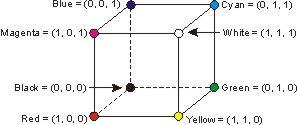
\includegraphics[scale=3]{color_cube}
\centering
\caption{RGB color model represented three-dimensionally using Cartesian coordinates.}
\centering
\end{figure}

\indent The RGB color model is an additive color model, where the primary colors are red, green, and blue. The secondary colors are cyan or a mixture of blue and green, magenta or red and blue, and yellow or red and green. The combination of the three primary additive colors produces white. Another model that is used in color printing is the CMY or CMYK model. This is a subtractive color model where the name stands for cyan, magenta, yellow, and black. The RGB model is good for digital images and color matching, but when printing, the three subtractive primary colors filter out red, green, and blue and make the pigmentation necessary to recreate images on paper.

\begin{figure}
\centering
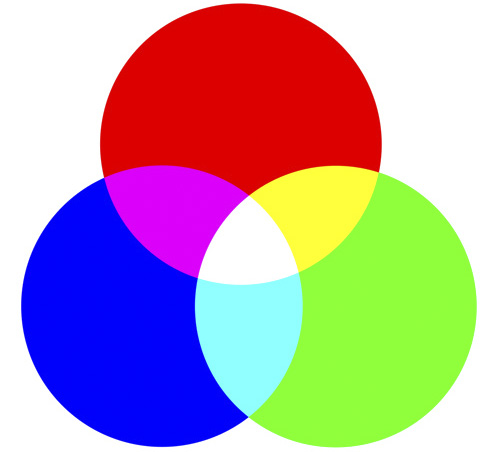
\includegraphics[scale=0.5]{color_space}
\caption{This is the average RGB color model representing the primary and secondary additive colors.}
\centering
\label{fig:my_label}
\end{figure}

\begin{figure}[!htb]
\centering
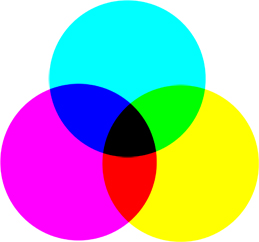
\includegraphics[scale=0.5]{cmyk}
\caption{stuff}
\centering
\label{fig:my_label}
\end{figure}

\section{Applications of color space}
\paragraph
\indent One of the most popular applications for color spaces is color photography. At first, to capture a photograph, the photographer would have to use paper treated with a light-sensitive substance like silver nitrite or silver chloride. The images that were produced were too faint or came out as negatives.The quality of the image is affected by the exposure time and the resin used on the paper. Reproducing images in color was the goal for a long time, and in 1848, a French physicist named Alexandre-Edmond Becquerel figured a way to make color images; however, the techniques were impractical due to long exposure times and short-lasting color, so it was rarely done. 

\section{Other factors of color}
\paragraph
\indent In this paragraph, I will discuss the hue, brightness, color intensities, and saturation, the HSI color model, and Newton's Hue Circle. 

\section{How we see color}
\paragraph
\indent In this paragraph, I will talk about the human eyes, and go in depth to how humans really see color. I will talk about light and wavelengths. I will also cite experiments done by physicists relating to light and color. I will also pose a question relating to color blindness and how animals such as dogs and cats see color.

\section{Theory of color vision and perception}
\paragraph
\indent In this paragraph, I will reference multiple theories on color, color perception, color blindness. I will look at Einstein, Newton, Maxwell, some psychology theories, and I will also look medical professionals on restoring color vision. 
\end{document}